\documentclass[10pt]{article}
\usepackage[a4paper,margin=18mm]{geometry}
\usepackage{amsmath,amssymb,booktabs,array,enumitem,longtable}
\usepackage[T1]{fontenc}\usepackage{lmodern}
\usepackage{tikz}\usetikzlibrary{shapes.gates.logic.US,positioning,arrows.meta,patterns,calc}
\usepackage[hidelinks]{hyperref}
\setlength{\parindent}{0pt}\setlength{\parskip}{4pt}\setlength{\emergencystretch}{2em}
\newcommand{\VDD}{V_{DD}}
\newcommand{\mos}[4]{\begin{scope}[shift={(#1,#2)}]
\draw (0,.24)--(0,-.24);\draw (0,.20)--(.25,.20)--(.25,.5);
\draw (0,-.20)--(.25,-.20)--(.25,-.5);\draw (-.16,.23)--(-.16,-.23);
\ifnum#4=1\draw (-.26,0) circle (.06);\draw (-.75,0)--(-.32,0);\else\draw (-.75,0)--(-.16,0);\fi
\node[anchor=east,font=\scriptsize] at (-.76,0) {$#3$};\end{scope}}
\newcommand{\ground}[2]{\draw (#1,#2)--(#1,{#2-.12});\draw ({#1-.17},{#2-.12})--({#1+.17},{#2-.12});\draw ({#1-.11},{#2-.20})--({#1+.11},{#2-.20});}
\newcommand{\rail}[3]{\draw (#1,#2)--(#1,{#2+.14});\node[above,font=\scriptsize] at (#1,{#2+.14}) {$#3$};}
\newcommand{\hmos}[4]{\begin{scope}[shift={(#1,#2)}]
\draw(-.24,0)--(.24,0);\draw(-.2,0)--(-.2,-.25)--(-.5,-.25);\draw(.2,0)--(.2,-.25)--(.5,-.25);
\draw(-.23,.16)--(.23,.16);
\ifnum#4=1\draw(0,.26)circle(.06);\draw(0,.32)--(0,.75);\else\draw(0,.16)--(0,.75);\fi
\node[below,font=\scriptsize]at(0,-.32){#3};\end{scope}}
\newcommand{\qheading}[1]{\par\medskip\textbf{#1}\par}
\begin{document}
\begin{center}{\Large\bfseries EE3032 Introduction to VLSI---Midterm}\\2012 archive attribution\end{center}
\small Complete editable reconstruction of seven questions from six green photographed panels, corresponding to three printed pages. The panel crops contain no printed date; 2012 is the archive-folder attribution. Point allocations total 100. This reconstruction contains the question text and figures, without student answer/identity pages.\normalsize
\qheading{1. (30 points) Complete the following problems briefly.}
\begin{enumerate}[label=(\alph*),leftmargin=7mm]
\item During the process of VLSI manufacture, chemical-mechanical polishing (CMP) is performed while a layer of material is grown. What is the purpose of CMP? (3 points)
\item The layer density rule should be met when you design a nano-scale IC. Why? (3 points)
\item What is the antenna effect? (3 points)
\item Draw a CMOS inverter and label the drain and source of the PMOS and NMOS transistors. (2 points)
\item Define the low and high noise margins of a CMOS inverter using the voltage transfer curve of the inverter. (3 points)
\item List two possible approaches for alleviating the effect of crosstalk on two neighboring parallel interconnects. (4 points)
\item List three major components of the load capacitance of a CMOS logic gate in a CMOS circuit. (3 points)
\item How do you size the N-type and P-type MOS transistors of an inverter such that the output voltage of the inverter is $V_{DD}/2$ when the input voltage is $V_{DD}/2$? (3 points)
\item List two types of FinFET structures. (3 points)
\item The delay of a long interconnection can be estimated by $k\ell^2$, where $k$ is a constant. What approach can be used to reduce the delay of interconnection? Explain your answer. (3 points)
\end{enumerate}
\qheading{2. (15 points)} Figure 1 shows a transistor-level schematic realizing a Boolean function $f$.
\begin{enumerate}[label=(\alph*),leftmargin=7mm]
\item Assume that the sizes of all PMOS transistors and NMOS transistors are the same and the turn-on resistance of PMOS and NMOS transistors is $R_p$ and $R_n$, respectively. Also, parasitic capacitances of nodes 1, 2, 3, and 4 are $C_1,C_2,C_3$, and $C_4$, respectively, and $C_1=C_2=C_3=C_4=C$. If functional inputs $(XYZ)$ of the circuit are $\{010,100,110,000,101,111\}$, calculate the worst-case rise time and fall time of the circuit using the Elmore RC delay model. (10 points)
\item Assume that the voltage swings at nodes 1, 2, 3, and 4 are $V_1,V_2,V_3$, and $V_4$. Also, the switching activities of nodes 1, 2, 3, and 4 are $\alpha_1,\alpha_2,\alpha_3$, and $\alpha_4$. If the logic operates at frequency $f$, express the internal cell power of the logic gate. (5 points)
\end{enumerate}
\begin{center}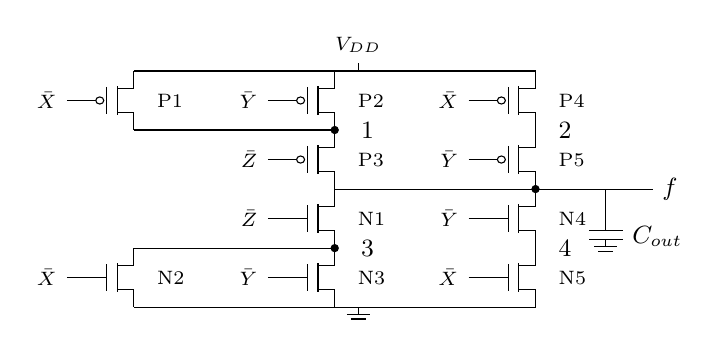
\begin{tikzpicture}[x=.85cm,y=.75cm,font=\small]
\mos{0}{6}{\bar X}{1}\mos{3}{6}{\bar Y}{1}\mos{3}{5}{\bar Z}{1}\mos{6}{6}{\bar X}{1}\mos{6}{5}{\bar Y}{1}
\draw(.25,6.5)--(6.25,6.5);\rail{3.6}{6.5}{V_{DD}}\draw(.25,5.5)--(3.25,5.5);\fill(3.25,5.5)circle(1.5pt);\node[right]at(3.5,5.5){1};\node[right]at(6.45,5.5){2};
\draw(3.25,4.5)--(8.0,4.5)node[right]{$f$};\fill(6.25,4.5)circle(1.5pt);
\mos{3}{4}{\bar Z}{0}\mos{0}{3}{\bar X}{0}\mos{3}{3}{\bar Y}{0}\mos{6}{4}{\bar Y}{0}\mos{6}{3}{\bar X}{0}
\draw(.25,3.5)--(3.25,3.5);\fill(3.25,3.5)circle(1.5pt);\node[right]at(3.5,3.5){3};\node[right]at(6.45,3.5){4};
\draw(.25,2.5)--(6.25,2.5);\ground{3.6}{2.5}
\foreach\x/\y/\n in {0/6/P1,3/6/P2,3/5/P3,6/6/P4,6/5/P5,3/4/N1,0/3/N2,3/3/N3,6/4/N4,6/3/N5}{\node[right,font=\scriptsize]at(\x+.45,\y){\n};}
\draw(7.3,4.5)--(7.3,3.8);\draw(7.05,3.8)--(7.55,3.8);\draw(7.05,3.65)--(7.55,3.65);\ground{7.3}{3.65}\node[right]at(7.55,3.7){$C_{out}$};
\end{tikzpicture}\\\small Figure 1: Transistor-level schematic.\end{center}
\newpage
\qheading{3. (10 points)} Figure 2(a) depicts a CMOS logic circuit in which the sizes of NMOS and PMOS for implementing each gate are the same. Assume that a dual-$V_t$ process can be used to implement the CMOS circuit. Draw the transistor schematic diagram of the CMOS circuit in terms of the symbols shown in Fig. 2(b) such that the leakage power of the CMOS circuit is minimal without sacrificing the speed of the CMOS circuit.
\begin{center}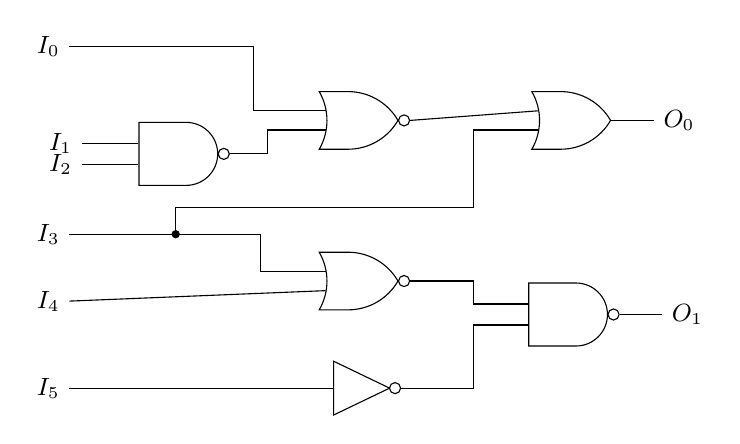
\begin{tikzpicture}[x=.9cm,y=.85cm,font=\small]
\node[nand gate US,draw,logic gate inputs=nn,minimum width=1cm](a)at(1.5,4){};
\node[nor gate US,draw,logic gate inputs=nn,minimum width=1cm](b)at(4,4.5){};
\node[or gate US,draw,logic gate inputs=nn,minimum width=1cm](o)at(7,4.5){};
\draw(a.input 1)--++(-.8,0)node[left]{$I_1$};\draw(a.input 2)--++(-.8,0)node[left]{$I_2$};\draw(a.output)--(2.8,4)|-(b.input 2);
\draw(0,5.6)node[left]{$I_0$}--(2.6,5.6)|-(b.input 1);\draw(b.output)--(o.input 1);\draw(o.output)--++(.6,0)node[right]{$O_0$};
\node[nor gate US,draw,logic gate inputs=nn,minimum width=1cm](e)at(4,2.1){};\node[not gate US,draw,minimum width=.8cm](v)at(4,.5){};\node[nand gate US,draw,logic gate inputs=nn,minimum width=1cm](g)at(7,1.6){};
\draw(0,2.8)node[left]{$I_3$}--(1.5,2.8)--(2.7,2.8)|-(e.input 1);\draw(1.5,2.8)--(1.5,3.2)--(5.7,3.2)|-(o.input 2);\fill(1.5,2.8)circle(1.5pt);
\draw(e.input 2)--(0,1.8)node[left]{$I_4$};\draw(v.input)--(0,.5)node[left]{$I_5$};\draw(e.output)--(5.7,2.1)|-(g.input 1);\draw(v.output)--(5.7,.5)|-(g.input 2);\draw(g.output)--++(.6,0)node[right]{$O_1$};
\end{tikzpicture}\quad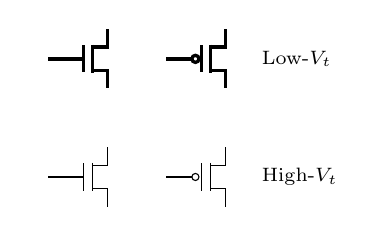
\begin{tikzpicture}[x=.75cm,y=.75cm,font=\scriptsize]
\begin{scope}[very thick]\mos{0}{2}{}{0}\mos{2}{2}{}{1}\end{scope}\mos{0}{0}{}{0}\mos{2}{0}{}{1}
\node[right]at(2.7,2){Low-$V_t$};\node[right]at(2.7,0){High-$V_t$};\end{tikzpicture}\\\small Figure 2: (a) A CMOS circuit (b) High- and low-$V_t$ transistor symbols.\end{center}
\qheading{4. (10 points)} Figure 3 shows a pass-transistor logic circuit. Assume that the supply voltage $V_{DD}=1.8$ V and the threshold voltage of the NMOS transistor is 0.4 V.
\begin{enumerate}[label=(\alph*),leftmargin=7mm]
\item Draw the corresponding waveforms at outputs $Y$ and $Z$ if the signal waveform shown in the leftmost figure is applied to input $X$. Note that you should label the largest and lowest values of voltage at the waveforms. (4 points)
\item Assume that the body effect of the transistors can be neglected. Also, the signal waveform shown in the leftmost figure is applied to input $X$.\\
i. Among the transistors $m1,m2,m3,m4,m5$, and $m6$, identify the transistors which can be operated in saturation and linear regions, and identify the transistor(s) which can be operated in the linear region only. Explain your answers. (6 points)
\end{enumerate}
\begin{center}\begin{tikzpicture}[x=.85cm,y=.8cm,font=\small]
\draw(-2,.75)--(-1.6,.75)--(-1.3,1.8)--(-.6,1.8);\node[left]at(-2,.75){0 V};\node[left]at(-2,1.8){1.8 V};
\draw(-.3,.75)node[left]{$X$}--(1,.75);\fill(.5,.75)circle(1.5pt);
\foreach\x/\n in {1.5/1,3/2,4.5/3,6/4,7.5/5,9/6}{\hmos{\x}{1}{$m_\n$}{0}\draw(\x,1.75)--(\x,2.2);}
\foreach\a/\b in {2/2.5,3.5/4,5/5.5,6.5/7,8/8.5}{\draw(\a,.75)--(\b,.75);}
\draw(1.5,2.2)--(9,2.2);\rail{6}{2.2}{V_{DD}}\draw(9.5,.75)--(10.2,.75)node[right]{$Z$};
\draw(10,.75)--(10,.35);\draw(9.8,.35)--(10.2,.35);\draw(9.8,.22)--(10.2,.22);\ground{10}{.22}
\hmos{3}{3}{}{0}\rail{3}{3.75}{V_{DD}}\hmos{6}{4.5}{}{0}
\draw(.5,.75)--(.5,4.25)--(5.5,4.25);\draw(.5,2.75)--(2.5,2.75);\fill(.5,2.75)circle(1.5pt);
\draw(3.5,2.75)--(4,2.75)--(4,5.25)--(6,5.25);\draw(6.5,4.25)--(8,4.25)node[right]{$Y$};
\draw(7.7,4.25)--(7.7,3.85);\draw(7.5,3.85)--(7.9,3.85);\draw(7.5,3.72)--(7.9,3.72);\ground{7.7}{3.72}
\end{tikzpicture}\\\small Figure 3: A pass-transistor logic circuit. The upper pass gate receives $X$ as data and a degraded copy of $X$ as its gate; it is not a two-device series data chain.\end{center}
\qheading{5. (10 points)} Figure 4 depicts an inverter chain driving a capacitive load $C_L$. Assume that the three inverters have the same size and every inverter has a minimum-size NMOS and the ratio of PMOS to NMOS is $\alpha$. Also, the $t_r$ and $t_f$ of an inverter driving a load $C_L$ can be estimated by $t_r=R_pC_L$ and $t_f=R_nC_L$, where $R_p$ and $R_n$ are the turn-on resistances of the PMOS and NMOS of the inverter. Let $\mu_n=3\mu_p$ and the turn-on resistance and gate capacitance of the minimum-size NMOS be $R$ and $C$, respectively. Derive the value of $\alpha$ such that $T=8RC$ and the average switching power contributed by the first two inverters is minimal.
\begin{center}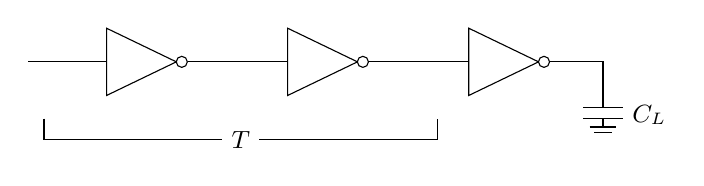
\begin{tikzpicture}[x=1cm,y=.9cm,font=\small]
\node[not gate US,draw,minimum width=1cm](i1)at(0,1){};\node[not gate US,draw,minimum width=1cm](i2)at(2.3,1){};\node[not gate US,draw,minimum width=1cm](i3)at(4.6,1){};
\draw(-1.3,1)--(i1.input);\draw(i1.output)--(i2.input);\draw(i2.output)--(i3.input);\draw(i3.output)--(6,1)--(6,.35);\draw(5.75,.35)--(6.25,.35);\draw(5.75,.2)--(6.25,.2);\ground{6}{.2}\node[right]at(6.25,.25){$C_L$};
\draw(-1.1,.2)--(-1.1,-.1)--(3.9,-.1)--(3.9,.2);\node[fill=white]at(1.4,-.1){$T$};
\end{tikzpicture}\\\small Figure 4: An inverter chain; $T$ brackets the first two inverter delays.\end{center}
\newpage
\qheading{6. (10 points)} Realize the following Boolean functions using static CMOS logic. You should show the transistor diagram.
\begin{enumerate}[label=(\alph*),leftmargin=7mm]
\item $f(w,x,y,z)=\overline{w(x+y+z)}$. (5 points)
\item $f(x,y)=\bar xy+x\bar y$. (5 points)
\end{enumerate}
Suppose that only true literals are available. Your implementation should use the minimal number of transistors.
\qheading{7. (15 points)} A full adder is a device that accepts three inputs $x,y$, and $c_{in}$ and produces two outputs $s_{out}$ and $c_{out}$, where $x,y,c_{in},s_{out}$, and $c_{out}$ denote the addend, augend, carry input, sum, and carry output, respectively.
\begin{enumerate}[label=(\alph*),leftmargin=7mm]
\item Derive the truth table for this full adder. (5 points)
\item From the truth table, derive the $s_{out}$ and $c_{out}$ Boolean functions. (5 points)
\item Realize it using CMOS logic circuit. (5 points)
\end{enumerate}
\vfill\small Original panels carry the course title and printed page identifiers 3-1, 3-2 and 3-3. No student annotations are added to the reconstructed prompts.\end{document}
